\clearpage
\section{Les supernovæ}


Les supernovae ont été introduite dans les simulations cosmologiques pour réduire l'effondrement du gaz sur lui même.
Sans l'introduction d'énergie dans le gaz par les supernovæ, le gaz s'effondre de manière importante et créer un nombre élevé d'étoiles.
Cela mène à un taux de formation stellaire trop important par rapport à ce qui est observé.
Ce problème est connus sous le nom de "overcooling problem"

L'objectif est de casser les structures pour diminuer les surdensité et limiter la formation stellaire.

%\subsection{Le modèle théorique}
%Il existe principalement deux événement pouvant mener a un explosion de supernovæ : 
%
%\begin{itemize}
%\item soit l'étoile est a l'origine suffisamment massive (plus de 8Mo) pour s'effondrer a la fin de sa vie.
%\item soit l'étoile n'est pas suffisamment massive (elle va donc mourir en naine blanche) mais dispose de suffisamment de matière a proximité (généralement étoiles double ou le compagnon pas en phase géante rouge) pour que sa masse augmente avec le temps.
%la matière accreté va faire passer la masse de cette étoile au dessus de la limite.
%\end{itemize}
%
%Les étoiles de plus de 8mo exploses en SN en injectant 1e51 erg dans le milieu\\
%Cette injection limite fortement la formation stellaire dans le milieu.\\
%modèle sous grille\\


Une fois que la supernovae a explosée, il en résulte une onde de choc qui va se propager dans le milieu environnant.

\subsection{Les différentes phases}
L'évolution du front d'onde à lieu en plusieurs phases, on en distinguera principalement deux : 

\begin{itemize}
\item Expansion adiabatique.
Dans la phase d'expansion adiabatique, l'énergie cinétique est conservée, le choc est violent et le gaz n'a pas le temps de perdre de l'énergie par radiation.
Dans cette phase, l'expansion est suffisamment rapide pour que la dissipation d'énergie par radiation soit négligeable.
%C'est le cas dans le test de Sedov.

\item Snowplow.
Dans la phase snowplow, le choc a suffisamment ralentis pour que le gaz commence à dissiper de l'énergie par rayonnement.
Dans ce cas, il se forme un bourrelet de compression dans lequel le gaz est poussé, comme dans le cas d'un chasse neige. 
Les pertes par radiation deviennent importantes et l'énergie cinétique n'est plus conservée
\end{itemize}

\subsection{Les Superbubles}

%A la manière de la percolation des bulles de HII, les bulles de supernovae 

Dans les endroits de formation stellaire, les étoiles ne sont pas isolées mais apparaissent ensemble au sein d'un même nuage de gaz.
L'effondrement gravitationnel du nuage mène a créer un génération D’étoile en un cours laps de temps.
Toutes ces étoiles vont mourir dans un laps de temps rapproché et ainsi, les différentes supernovæ vont injectée de l’énergie dans le milieu dans un temps très rapproché.
Les différentes bulle vont se rencontrer (à la manière des bulles ionisées) et mener à une bulle plus grande appelée superbubble.

\subsection{Considérations d'échelles}
La façon de gérer les supernovae sera donc fonction de l'échelle que l'on considère.
Dans des simulations très détaillées de galaxies, il sera nécessaire de résoudre la phase adiabatique d'explosion individuelle.
Dans des simulations cosmologiques de la réionisation, L’intérêt sera plus porté sur la phase snowplow des superbubbles.

%\subsection{ Différentes implémentations existantes}
%\subsubsection{Navaro and white}
%\subsubsection{Stinson et al}
%\subsubsection{dubois et Teyssier}
%Utilisation de particule fantômes pour simuler les différentes phase
%
%\subsubsection{Dalla Veccia et Schaye}
%Modèle probabiliste, injection d'énergie seulement si l'énergie est suffisante pour générer un mouvement suffisant.

\subsection{Mes Implémentations}
\label{sec:SNmodel}

\subsubsection{Modèle thermique}
Le modèle thermique consiste a injecter l’énergie sous forme d’énergie interne.
Il existe 2 variables d’état liées a l’énergie interne: la pression et la température, modifier l'une de ces variables est équivalent.
Dans l’implémentation actuelle, le choix a été fait de travailler sur la pression.
Elle est modifiée en utilisant cette conversion:

\begin{equation}
P^{0+} = P^{0-}  + E_0 * (\gamma-1)
\end{equation}

Ce modèle est connu pour avoir de fortes pertes de d'énergie dans le cas ou le refroidissement est autorisé.


\subsubsection{le model cinetique}


\begin{figure}
        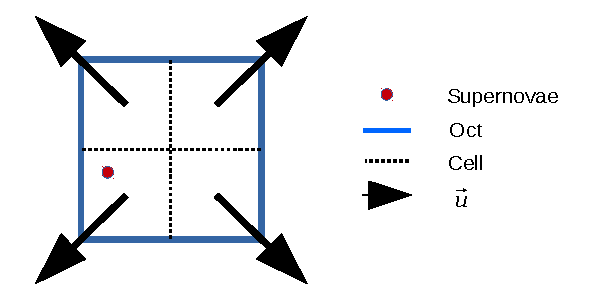
\includegraphics[width=.95\linewidth]{img/03/oct_kinetic.pdf} 
        \caption{
 		\label{fig:kin}}
\end{figure}
Le modèle cinétique consiste a modifier directement la vitesse du gaz autour de l'explosion dans le but de shunter la conversion de l'énergie interne en mouvement.
Ce type de model a été utilisé pour 

Nous avons fait le choix de limiter le nombre de cellules utilisées a 8 correspondant a 1 oct de la structure AMR d'\emma

\begin{equation}
e_{SN} = E_{SN}/8
\end{equation}

Ensuite cette énergie est utilisé pour changer la vitesse du gaz en utilisant : 
\begin{equation}
    \Delta \overrightarrow{v_{gas}} = \sqrt{\frac{2e_{SN}}{\rho_g.dV}} \overrightarrow{u}
    \label{eq_sn_direct}
\end{equation}


\subsection{Test numérique (Sedov)}
\label{sec:sedov}

%la dérivation des solutions du test de Sedov se trouve :
%chapitre 17 de Shu the physique of astrophysic Volume 2.\\

Dans le but de tester l'implémentation des différents modèles d'injection d'énergie, je l'es ai soumis au test de Sedov.
Ce test est utilisé pour tester le cas d'une explosion parfaite.
Il consiste a relâcher instantanément une quantité d'énergie $E_0$ dans un milieu homogène d'indice adiabatique $\gamma$, de densité $\rho_0$ et de pression $P_0$ (ou de température $T_0$).
Ce brusque changement dans l'état du système créer une discontinuité que le solveur va devoir gérer.

L'avantage de ce test est qu'il dispose d'une solution analytique.
Sedov a exprimé  en 1959 que le rayon de l'explosion en fonction du temps peux s'exprime : %TODO ref

\begin{equation}
r_{(t)}=\left( \frac{E_0}{\alpha \rho_0 }\right)^{1/5} t^{2/5}
\end{equation}


\subsubsection{Sedov évolution temporelle }


parametre du test :
rho=1
p=1e-5
v=0
gamma=5/3


Ce test consiste a suivre l'onde de choc et a s'assurer que son profil et sa position sont correct dans le temps.
On calcul pour chaque cellule sa distance au centre de l'explosion, puis en utilisant un histogramme sur les rayons, pondéré par la valeur du champ que l'on veux analyser, on obtient rapidement le profil radial moyen.
Le résultats présentés utilise l'injection thermique simple (dans une seule cellule).

Le domaine de calcul est en une grille régulière décomposé en $256^3$ éléments  de calcul et le raffinement n'est pas autorisé.

La Fig. \ref{fig:sedov_evol} présentes le trois principaux champs (densité, pression et vitesse radiale) a trois instant différents, comparé a la solution analytique.
On observe un très bon accord en la simulation et le théorie.
Notre méthode d'injection d'énergie est correcte et bien dimensionnée.
%
%\begin{figure}[bth]
%        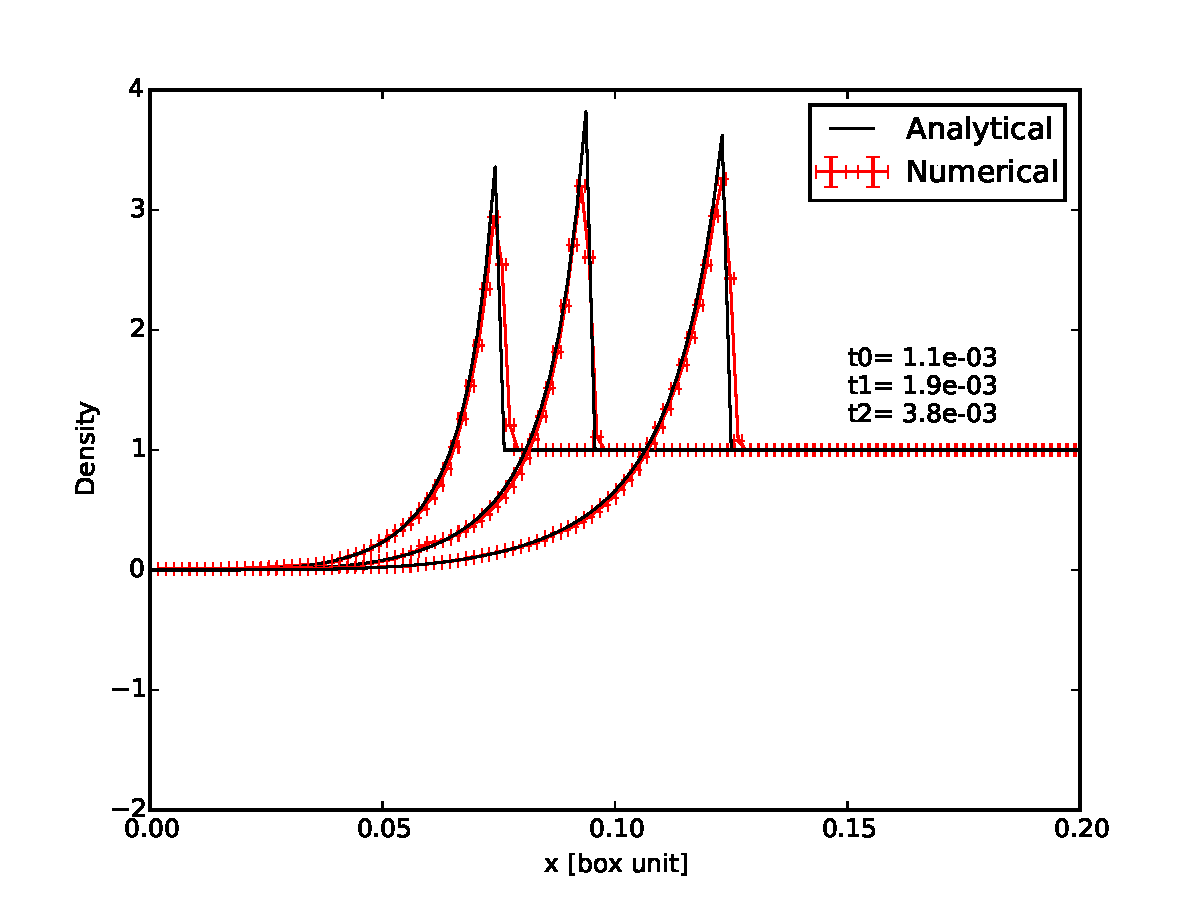
\includegraphics[height=.3\textheight]{img/03/sedov/sedov_evol_8_den_lin.pdf} 
%		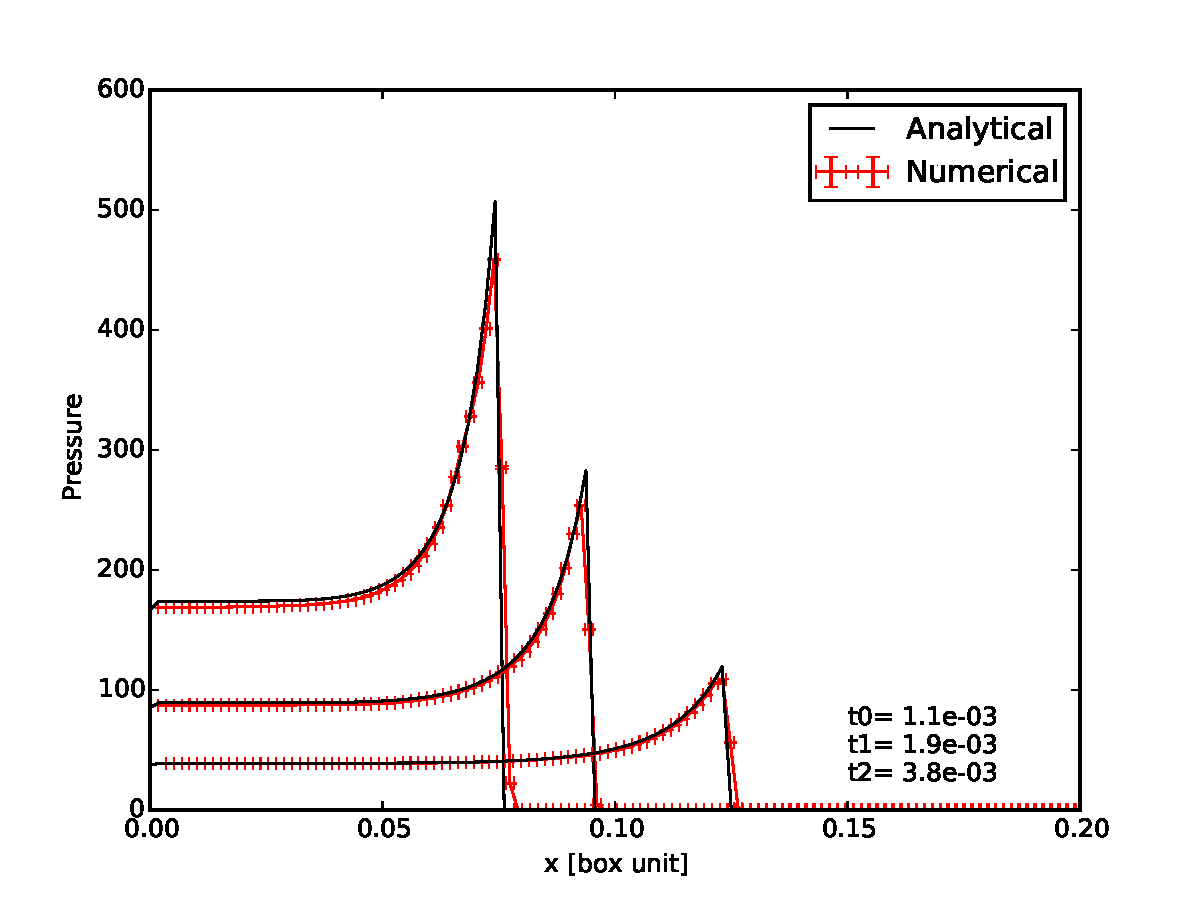
\includegraphics[height=.3\textheight]{img/03/sedov/sedov_evol_8_pres.pdf} 
%		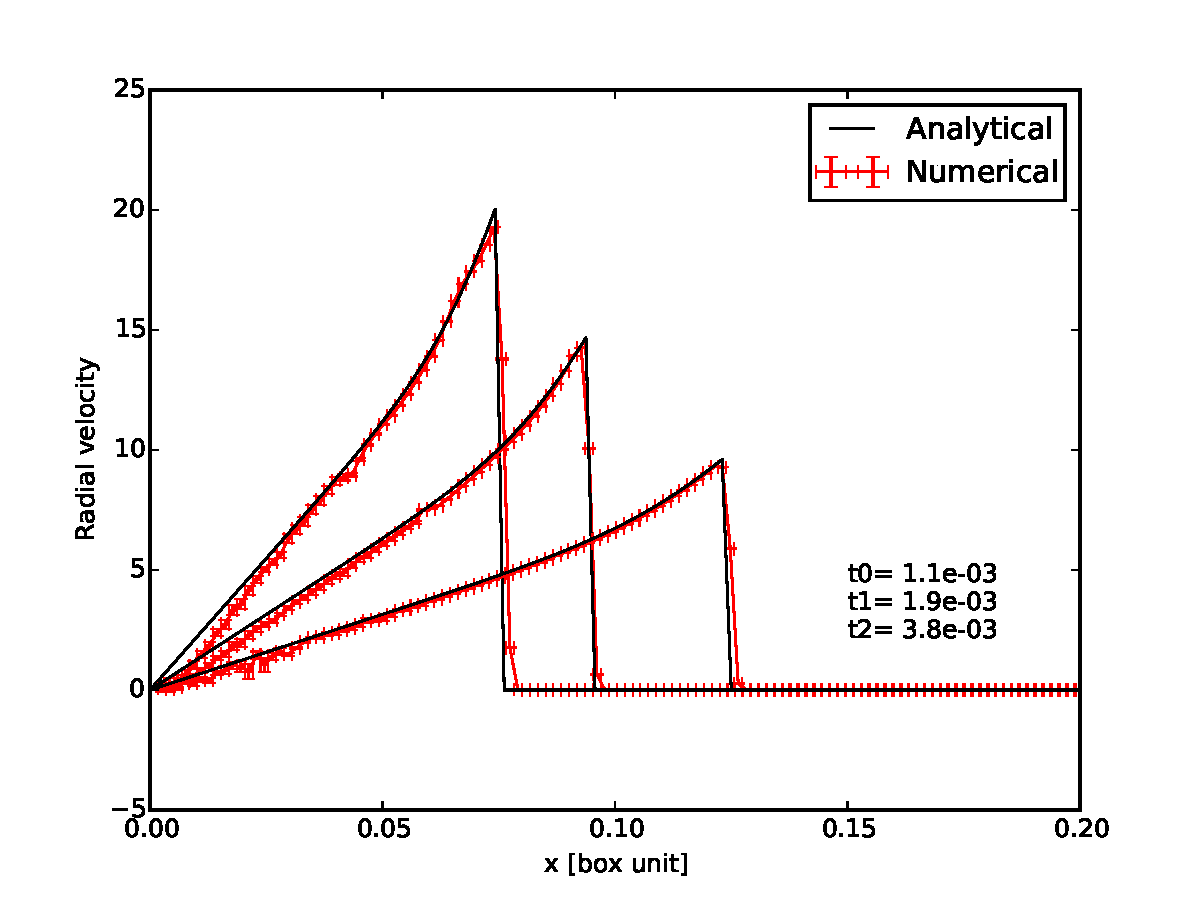
\includegraphics[height=.3\textheight]{img/03/sedov/sedov_evol_8_vel.pdf} 
%        \caption{Test de Sedov, évolution des différentes variables d'états. La densité en haut, la pression au milieu et la vitesse radiale en bas.}
% 		\label{fig:sedov_evol}
%\end{figure}

\begin{figure}[bth]
   \begin{minipage}[c]{.46\linewidth}
        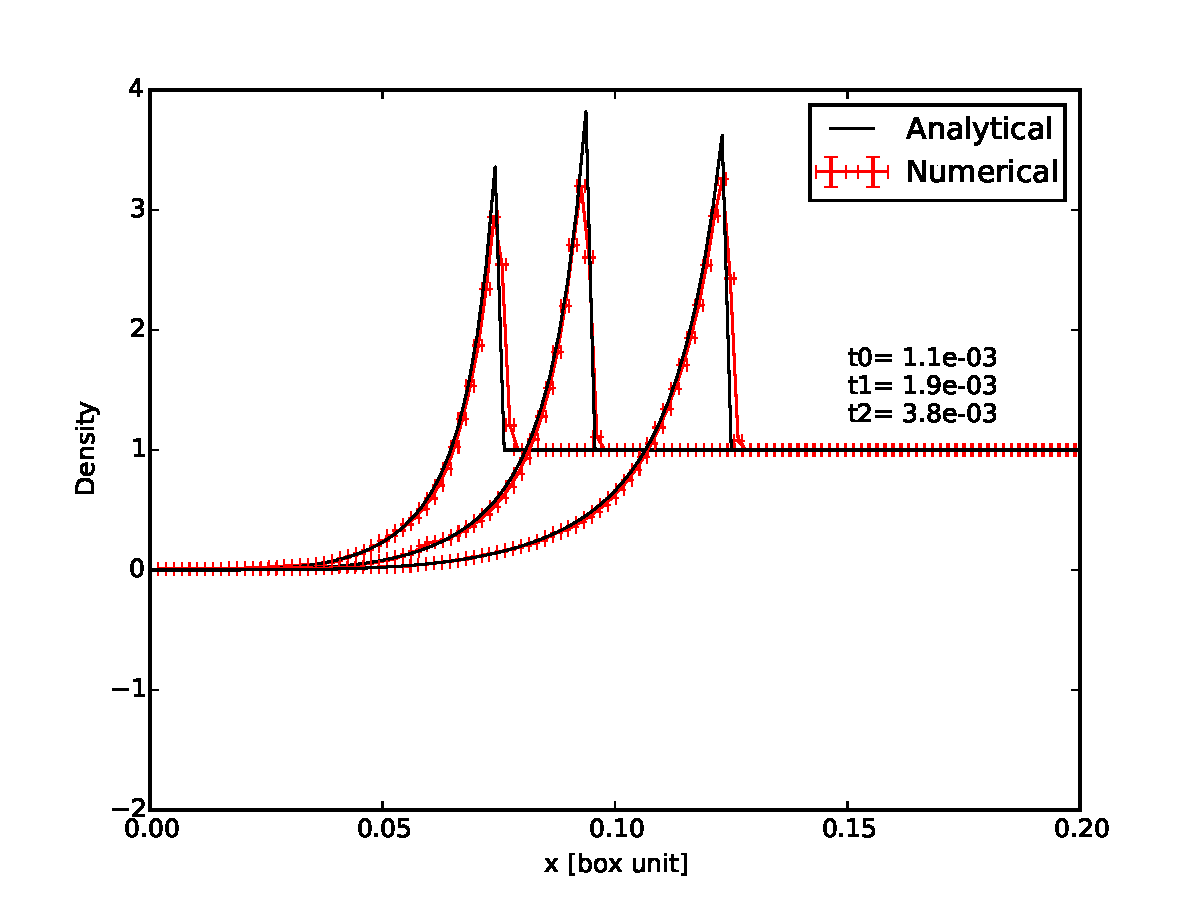
\includegraphics[width=\textwidth]{img/03/sedov/sedov_evol_8_den_lin.pdf} 
		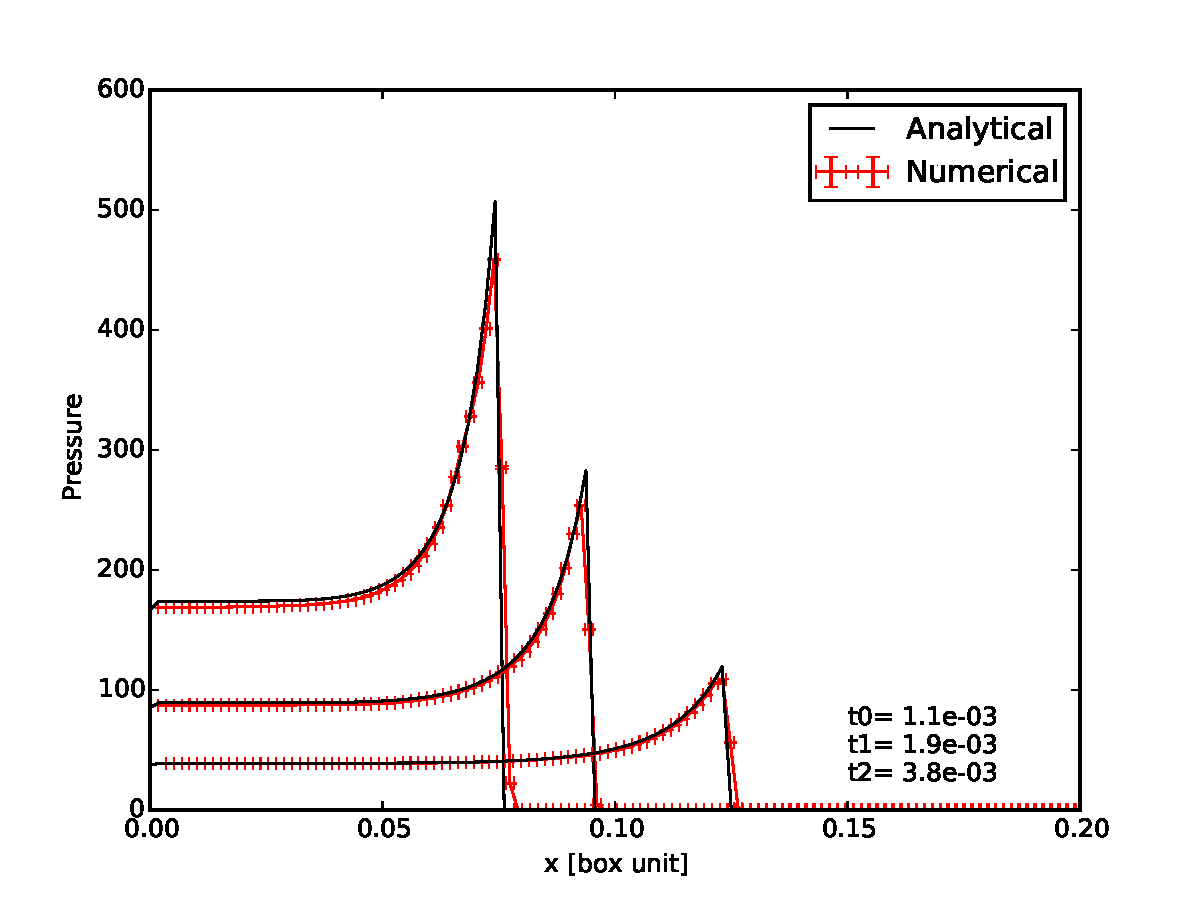
\includegraphics[width=\textwidth]{img/03/sedov/sedov_evol_8_pres.pdf} 
		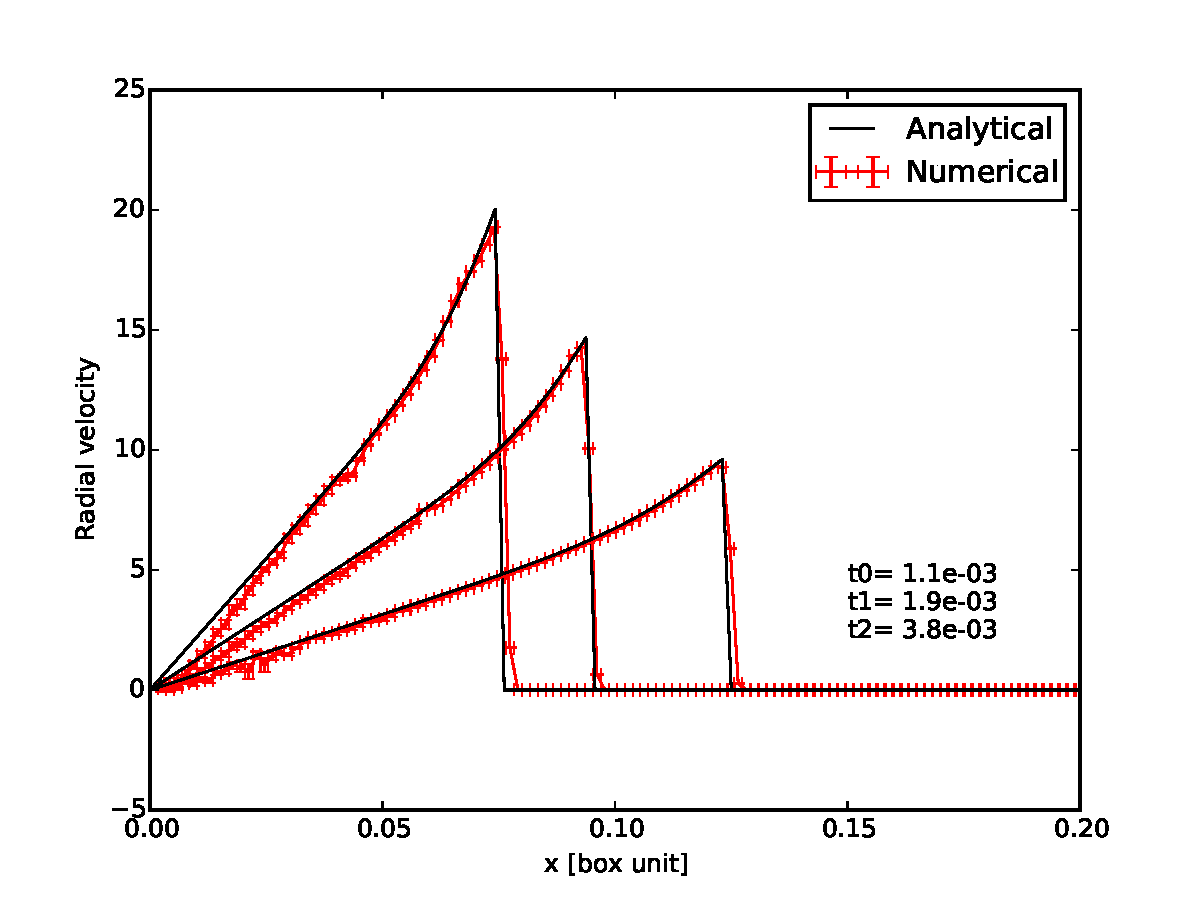
\includegraphics[width=\textwidth]{img/03/sedov/sedov_evol_8_vel.pdf} 

   \end{minipage} \hfill
   \begin{minipage}[c]{.46\linewidth}
		
		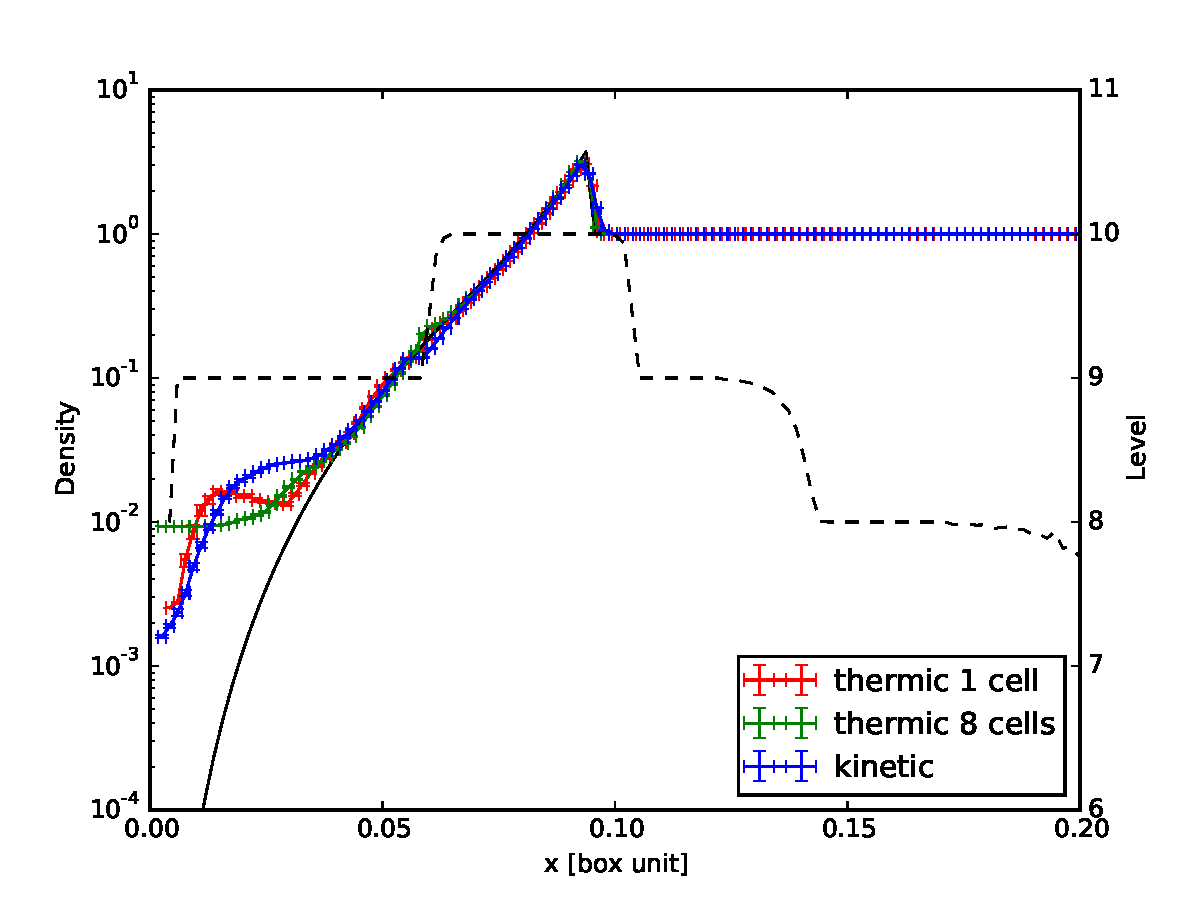
\includegraphics[width=\textwidth]{img/03/sedov/sedov_comp_profile_den.pdf} 
		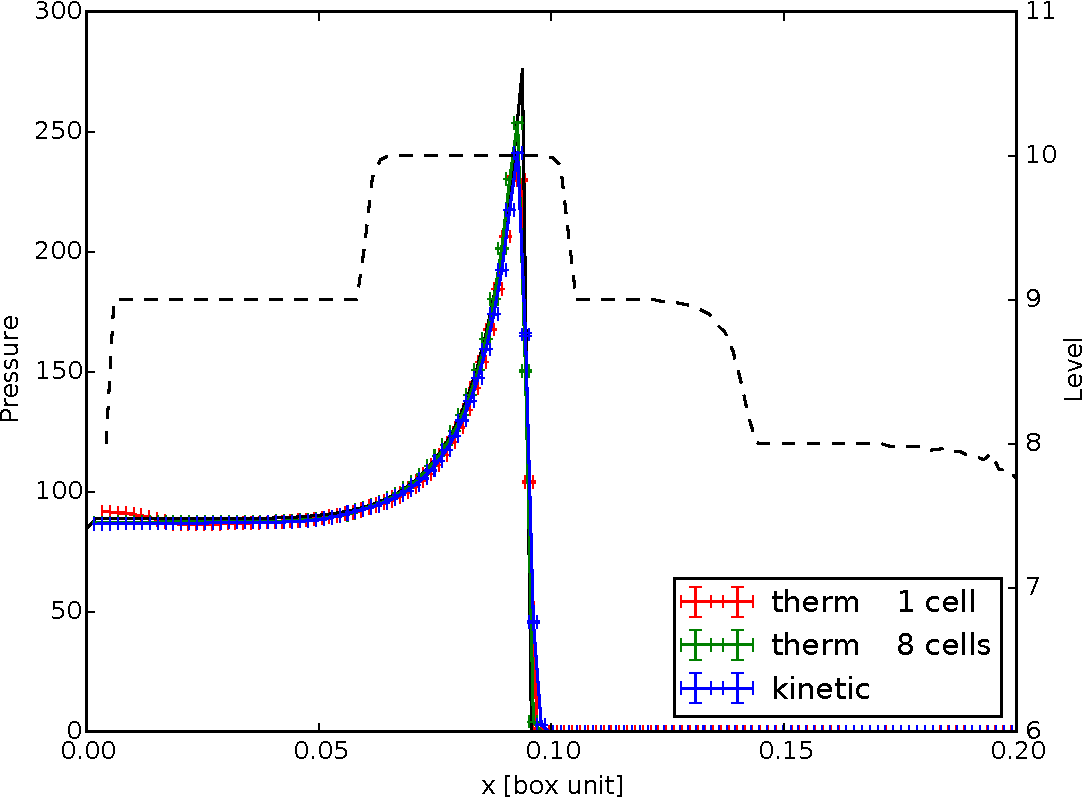
\includegraphics[width=\textwidth]{img/03/sedov/sedov_comp_profile_pres.pdf} 
		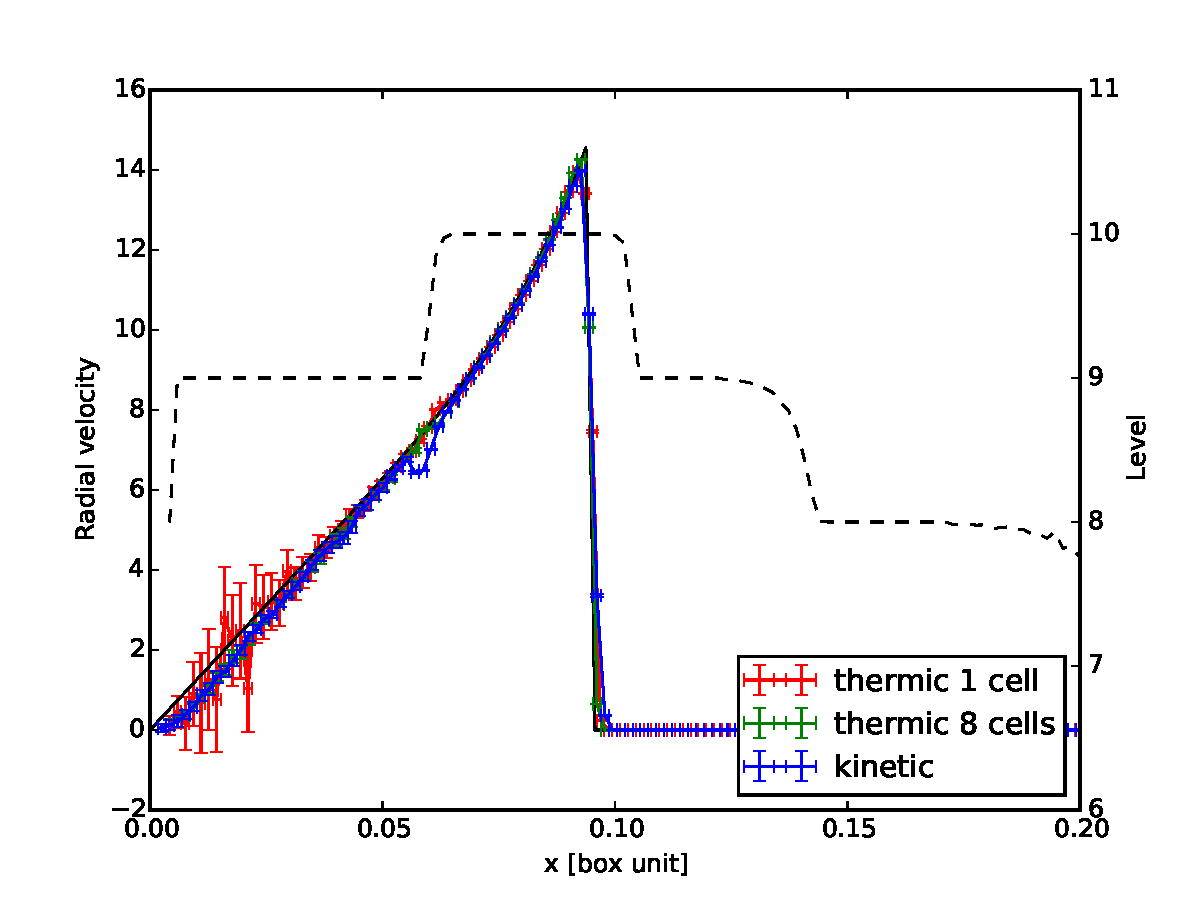
\includegraphics[width=\textwidth]{img/03/sedov/sedov_comp_profile_vel.pdf} 

   \end{minipage}

        \caption{Test de Sedov, évolution des différentes variables d'états. La densité en haut, la pression au milieu et la vitesse radiale en bas.        
        Test de Sedov, comparaison des profil radial en fonction des  méthodes d'injection. 
        Densité en haut, pression au milieu et vitesse radial en bas.
        La position et la forme du front d'onde ne dépendent pas de la méthodes d'injection utilisée.
% 		\label{fig:sedovmethod} 
 		}
 		\label{fig:sedov_evol}
\end{figure}



\subsubsection{Sedov comparaison entre les méthodes}

Nous avons vu qu'il existe différents moyens d'injecter de l'énergie dans le solveur hydrodynamique.
Le test présenté ici consiste a vérifié que les différentes méthodes sont équivalentes entre elles.

Nous allons comparer 3 méthodes : 
\begin{itemize}
\item l'injection thermique dans une cellule 
\item l'injection thermique dans un cube de huit cellules
\item l'injection cinétique  dans un cube de huit cellules
\end{itemize}


Ces 3 tests utilisent cette fois ci espace discret de  $128^3$ éléments, mais en autorisant le raffinement sur 3 niveaux.
Le raffinement est effectué sur le gradient de densité, ie une cellule est divisé si le gradient de densité qu'elle contient est supérieur a une certaine valeur.
Cette méthode permet de concentrer le raffinement sur le front de l'onde choc.

La figure \ref{fig:sedovraff} présente le motif de raffinement obtenu pour le test d'injection thermique sur une cellule.
Tout les tests présentent un motif de raffinement similaire.

%\begin{figure}[htpb]
%        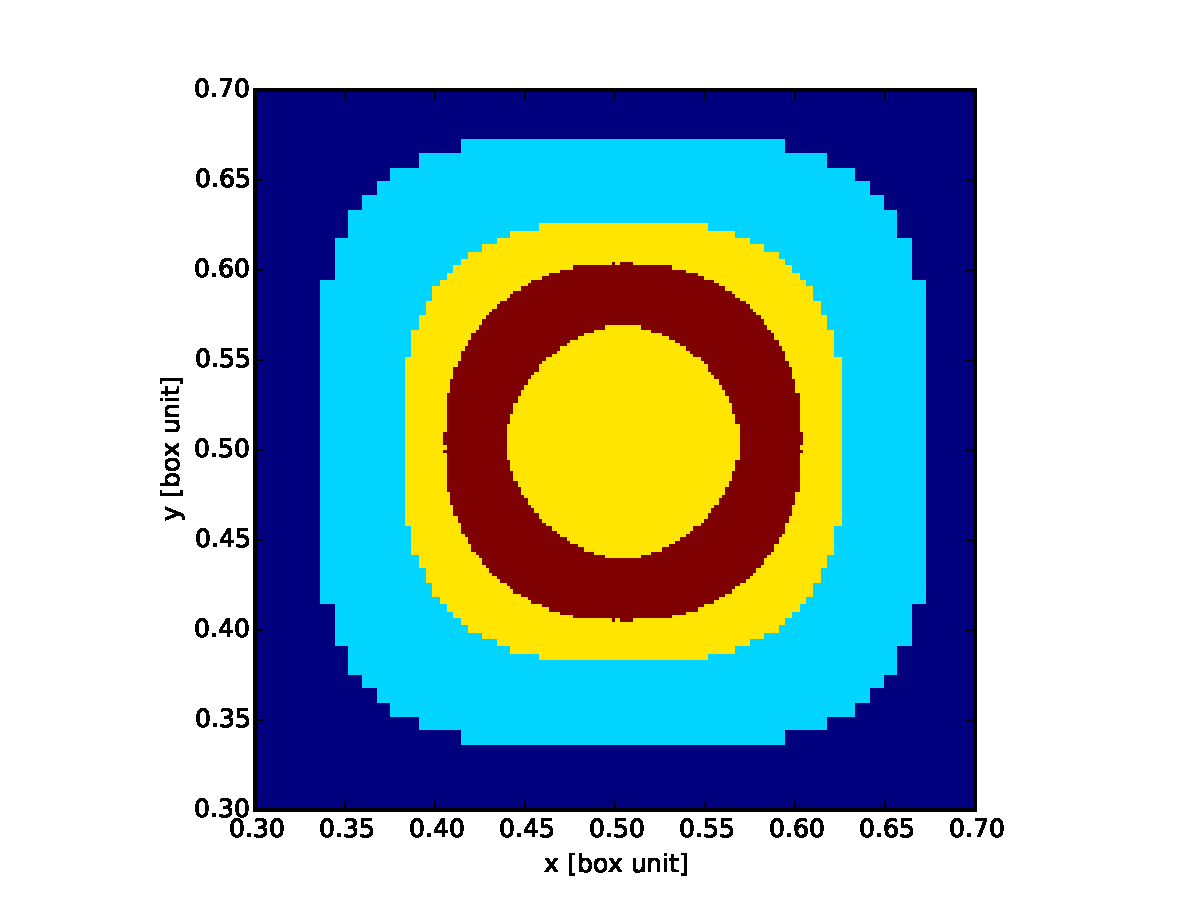
\includegraphics[width=.95\linewidth]{img/03/sedov/slice_th_1raf.pdf} 
%        \caption{Test de Sedov, raffinement (mettre la color map) }
% 		\label{fig:sedovraff}
%\end{figure}

La figure \ref{fig:sedovmethod} presente les profils obtenus a un instant donné pour les différentes méthodes d'injection d'énergie et pour les différents champs.
On observe que le front est bien situé au même endroits indépendamment de la méthode.
%Le profil de densité est présenté en échelle logarithmique pour accentuer les difference au niveau du centre. 

%\begin{figure}[htpb]
%        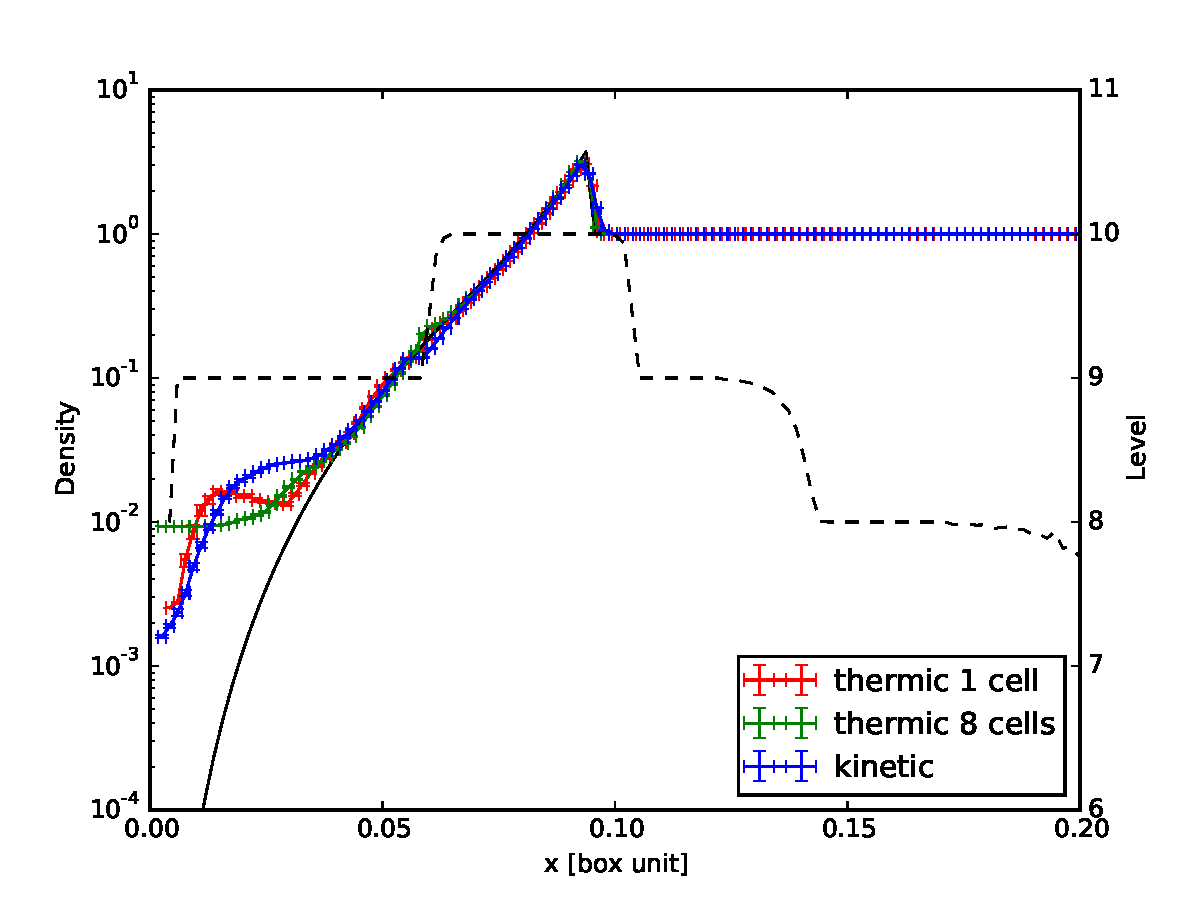
\includegraphics[height=.3\textheight]{img/03/sedov/sedov_comp_profile_den.pdf} 
%		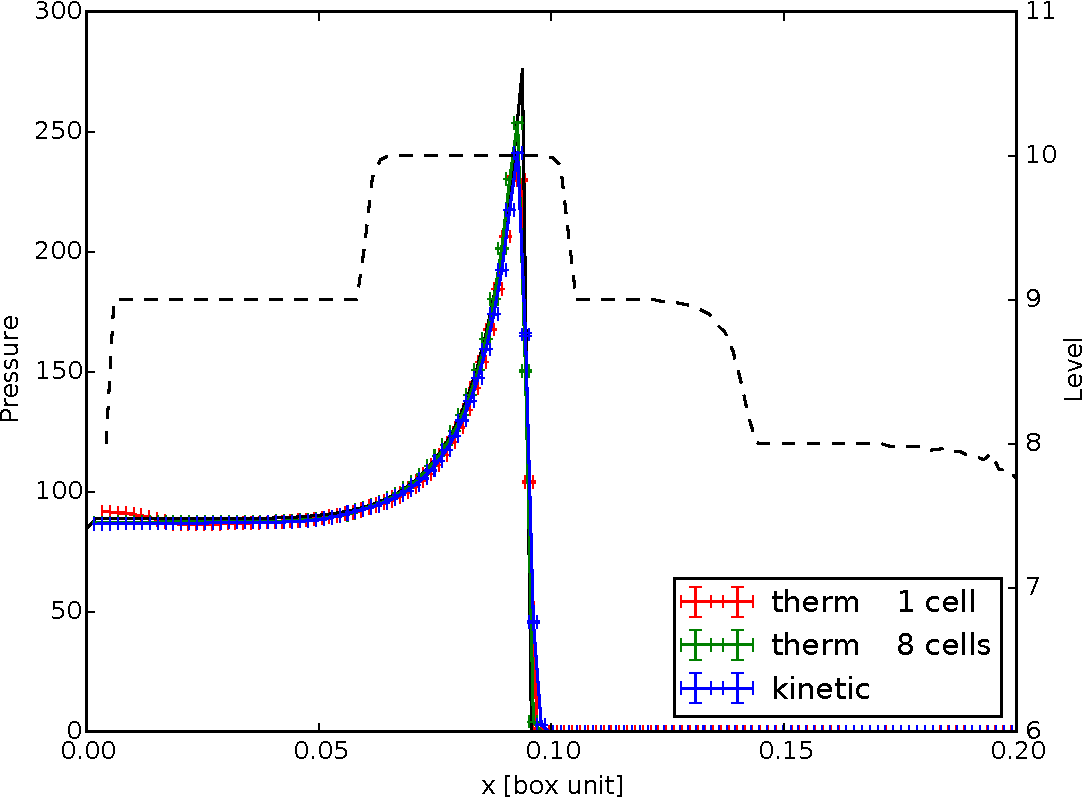
\includegraphics[height=.3\textheight]{img/03/sedov/sedov_comp_profile_pres.pdf} 
%		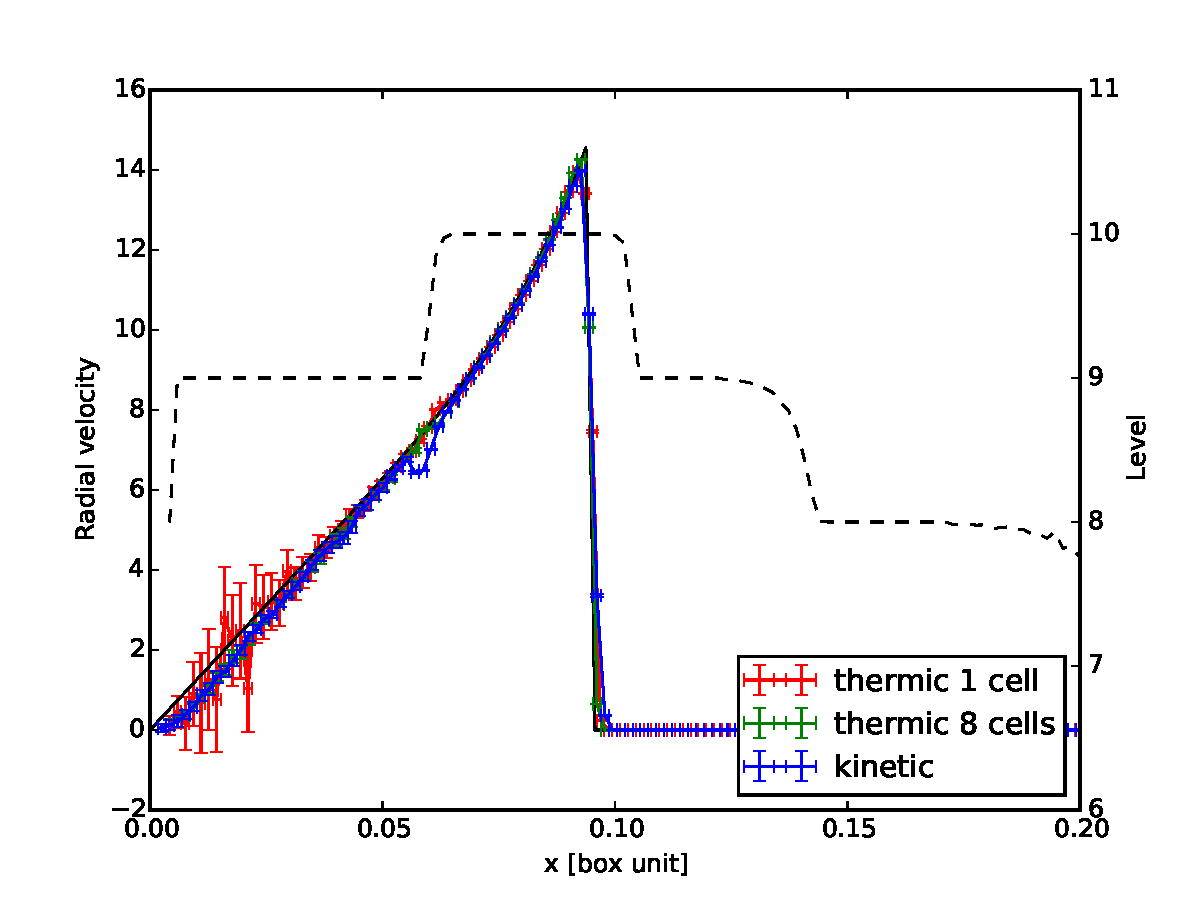
\includegraphics[height=.3\textheight]{img/03/sedov/sedov_comp_profile_vel.pdf} 
%        \caption{Test de Sedov, comparaison des profil radial en fonction des  méthodes d'injection. 
%        Densité en haut, pression au milieu et vitesse radial en bas.
%        La position et la forme du front d'onde ne dépendent pas de la méthodes d'injection utilisée.}
% 		\label{fig:sedovmethod} 
%\end{figure}


Même si les profils radiaux moyens sont comparables, on observe des différences sur la forme de l'explosion.
La figure \ref{fig:sedovslice} présente une coupe suivant l'axe z de la grille, contenant la cellule d'injection, pour les trois méthodes.
Ces différence sont dues a la grille et a la façon dont les flux sont calculés.
Dans le cas de l'injection thermique, les flux auront tendance à être suivant les axes principaux de la grille.
Ce qui donne ce motif en forme de "+" bien particulier.
Dans le cas de l'injection cinétique, les sont forcés a être dans des directions obliques, a 45°, par rapport a la l'axe de la grille.
Nous avons cette fois si une figure en forme de "x".

%\begin{figure}[htpb]
%        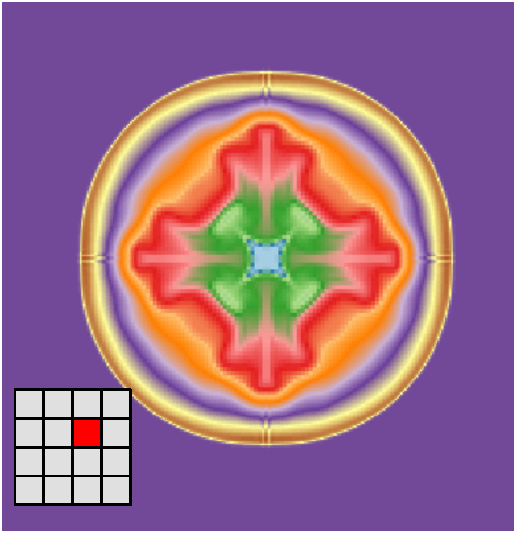
\includegraphics[height=.3\textheight]{img/03/sedov/slice_therm1.pdf} 
%		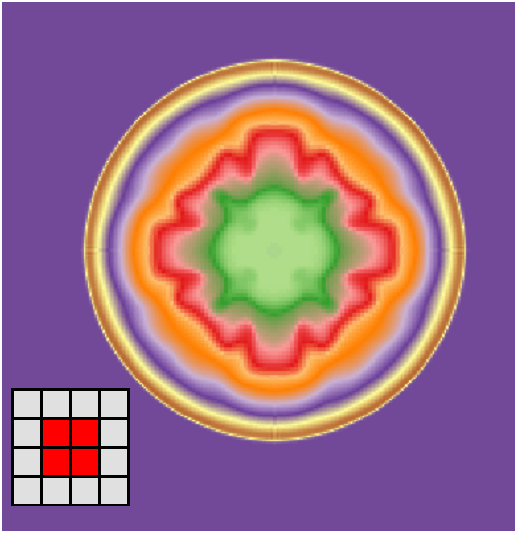
\includegraphics[height=.3\textheight]{img/03/sedov/slice_therm4.pdf} 
%		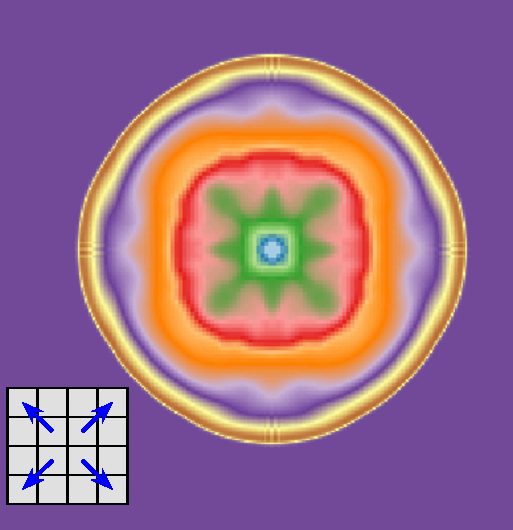
\includegraphics[height=.3\textheight]{img/03/sedov/slice_kin.pdf} 
%        \caption{Test de Sedov}
% 		\label{fig:sedovslice}
%\end{figure}



\begin{figure}[htpb]

	\centering
	\subfloat[]{        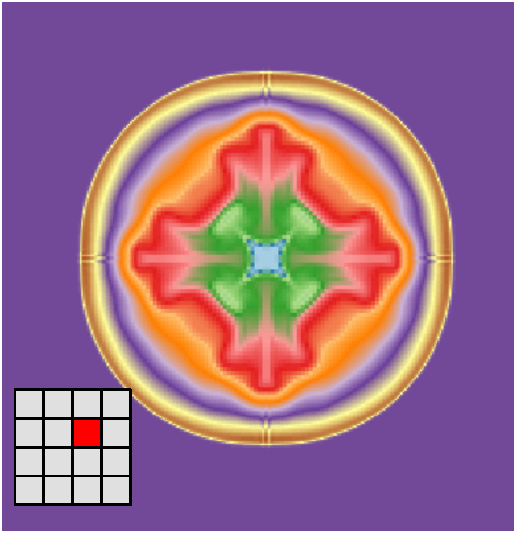
\includegraphics[width=.45\linewidth]{img/03/sedov/slice_therm1.pdf}} 
	\subfloat[]{		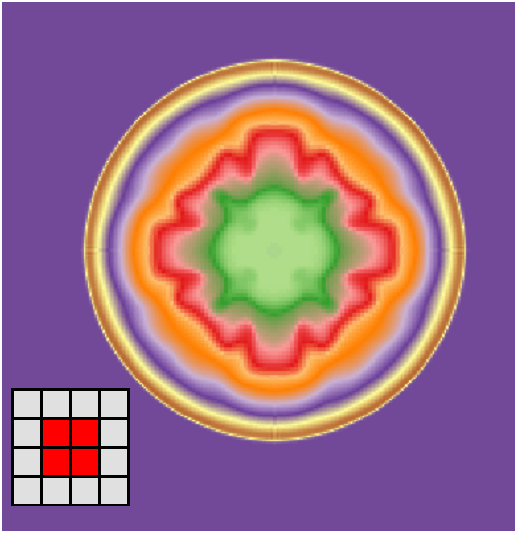
\includegraphics[width=.45\linewidth]{img/03/sedov/slice_therm4.pdf}} \\

	\subfloat[]{		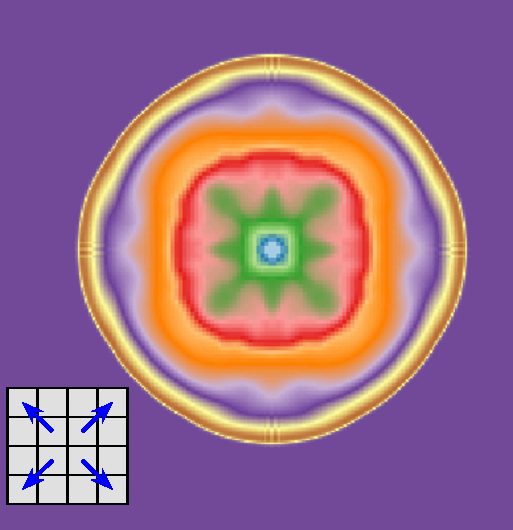
\includegraphics[width=.45\linewidth]{img/03/sedov/slice_kin.pdf} }
	\subfloat[]{		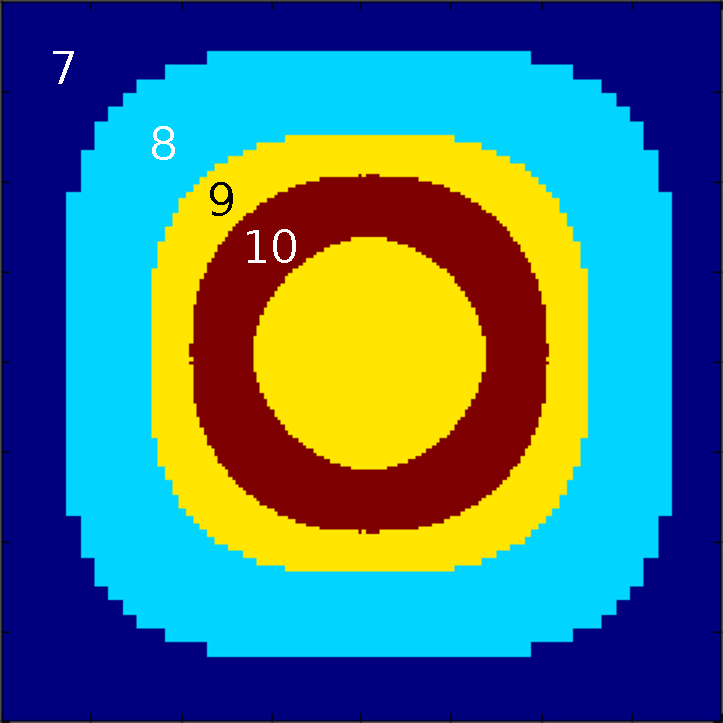
\includegraphics[width=.45\linewidth]{img/03/sedov/slice_th_1raf_cut.pdf}  }

    \caption{Différents motif d'explosion en fonction de la méthodes d'injection.
    Chaque figure représente une tranche d'une cellule d'épaisseur contenant le site de l'explosion.
    (a), (b) et (c) représente le log de la densité avec une colormap quantitative.
    A cause de la grille de calcul, il existe des axes privilégiés pour les flux, il en résulte des motif en croix et ou en losange.
    La figure (d) représente les niveaux de raffinements, le niveau 10 est aligné sur le front d'onde.
    }
 	\label{fig:sedovslice}
\end{figure}



\subsubsection{Conclusion}

La conclusion de ses tests est que les différentes méthodes d'injection sont équivalentes, au moins dans le contexte du test de Sedov.

%OK\\
%mais pas en cosmo

le pas de temps\\


\section{Tests en conditions de production}

Dans le but de tester ces différentes méthodes d'injections dans un contexte cosmologique j'ai réalisé une série de simulations.
Chacune de ces simulation est strictement identique a l'exception de la méthode d'injection d'énergie.
Les paramètres communs a toutes les simulations qui vont suivre sont les suivants:

Elles représentes un volume de 8/h cMpc cube échantillonnées par 256 cube particules de matière noire.
Ce sui mène a une résolution en masse de 3.4 10 6 M0 et une résolution spatiale de 46 ckpc sur la grille coarse.
La grille est raffinée suivant une méthode semi lagrangienne (voir Sec. \ref{sec:raffinement}).

Les condition initiales ont été générées avec MUSIC avec une cosmologie de Planck \citep{planck_collaboration_planck_2016} : 
$\Omega_m=0.3175$, 
$\Omega_v=0.6825$,
$\Omega_b=0.0490$,
$H_0=67.11$,
$\sigma_8=0.830$. 
Les simulations commences a redshift z=150.


Le premier test consiste a essayer les différents feedback avec la même quantité d'énergie injectée, et a mesurer leur impact sur la SFH cosmique.
La figure \ref{fig:sfr_methode} présente les résultats obtenus.
La méthode d'injection cinétique a plus d'impact en condition cosmologique.
Ceci est du a l'introduction de la physique du refroidissement.
La méthode thermique repose sur le principe de conversion de l'énergie interne en énergie cinétique.
La méthode thermique est connue %TODO ref
pour subir d'importante perte d'énergie.
La méthode cinétique outre passe cette conversion et mets directement le gaz en mouvement.

%TODO parler du feedback radiatif

\begin{figure}[bth]
        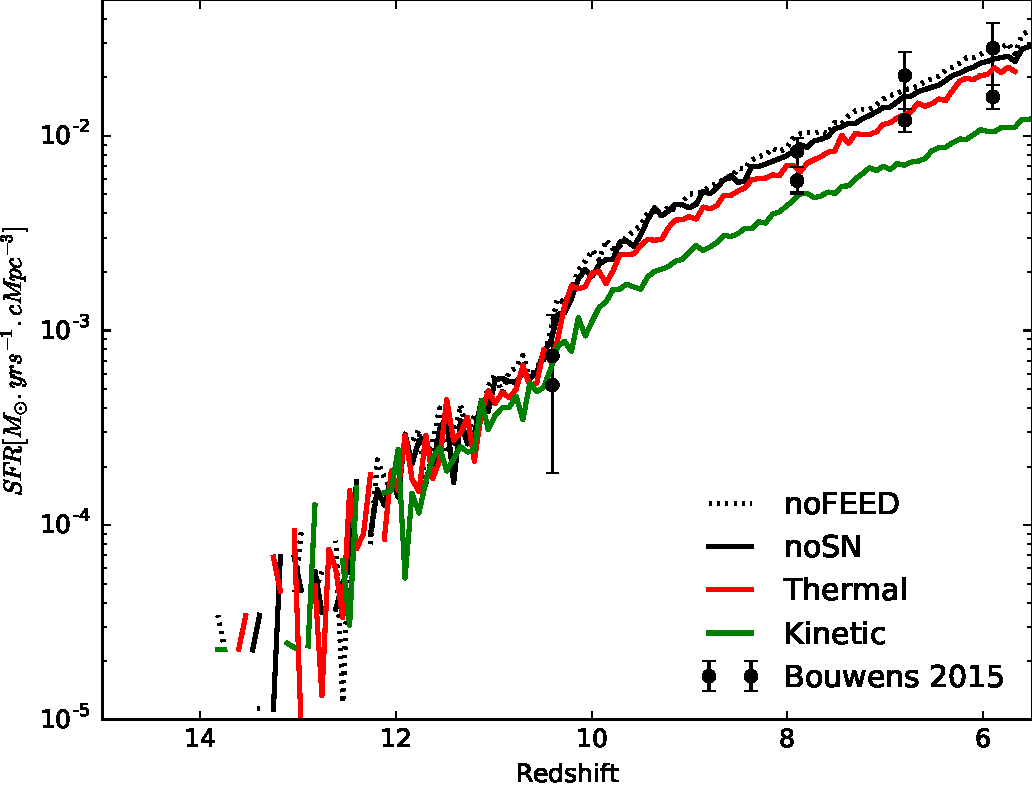
\includegraphics[width=.95\textwidth]{img/03/sedov/SFRmethode.pdf} 
        \caption{SFH cosmique en fonction de la méthode d'injection.
        Les méthodes n'impactent pas le milieu de la même manière
        }
 		\label{fig:sfr_methode}
\end{figure}

Nous aurons donc tendance préférer la méthode cinétique par la suite, vu que celle ci est plus efficace a nos échelles.
Le deuxième test consiste a utilisé la méthode cinétique et a varier la quantité d'énergie injectée.
La figure \ref{fig:sfr_egy} présente les résultats obtenus.
On y observe que plus on injecte d'énergie, plus la SFR instantanée diminue.
Ce qui est le comportement attendus puisque plus les supernovae sont puissante, plus les sur-densités de gaz sont "cassées", et donc plus difficile il devient de former de nouvelles étoiles.

\begin{figure}[bth]
        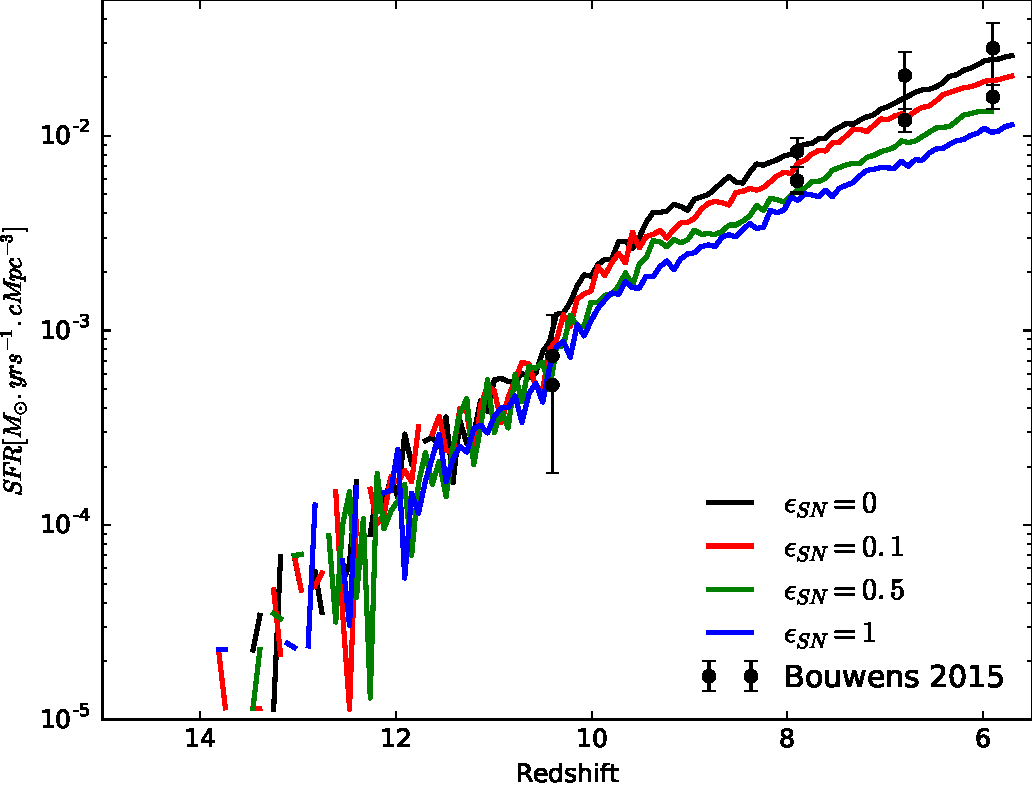
\includegraphics[width=.95\textwidth]{img/03/sedov/sneff_SFR.pdf} 
        \caption{SFH cosmique en fonction de la quantité d'énergie injectée. 
        Plus la quantité d'énergie injecté est importante, plus le taux de formation stellaire diminue.
        }
 		\label{fig:sfr_egy}
\end{figure}



Un troisième test consiste a injecter une certaine quantité d'énergie par supernovae, et a faire varier l'efficacité de formation stellaire.
En effet plus on forme d'étoiles et plus le feedback devient important, mais plus il y a de feedback, moins il est facile de former de nouvelles étoiles.
Le couplage entre feedback et formation stellaire n'est pas clair et mérite d'être exploré.
La figure \ref{fig:sfr_sfe} présente ce test pour trois efficacité de formation stellaire avec un modèle de feedback cinétique et une efficacité de supernovae de 100 \%.
On observe un fort couplage entre feedback et formation stellaire, a tel point que pour une efficacité de formation stellaire de 10\% le feedback mène a une SFH décroissante.

\begin{figure}[bth]
        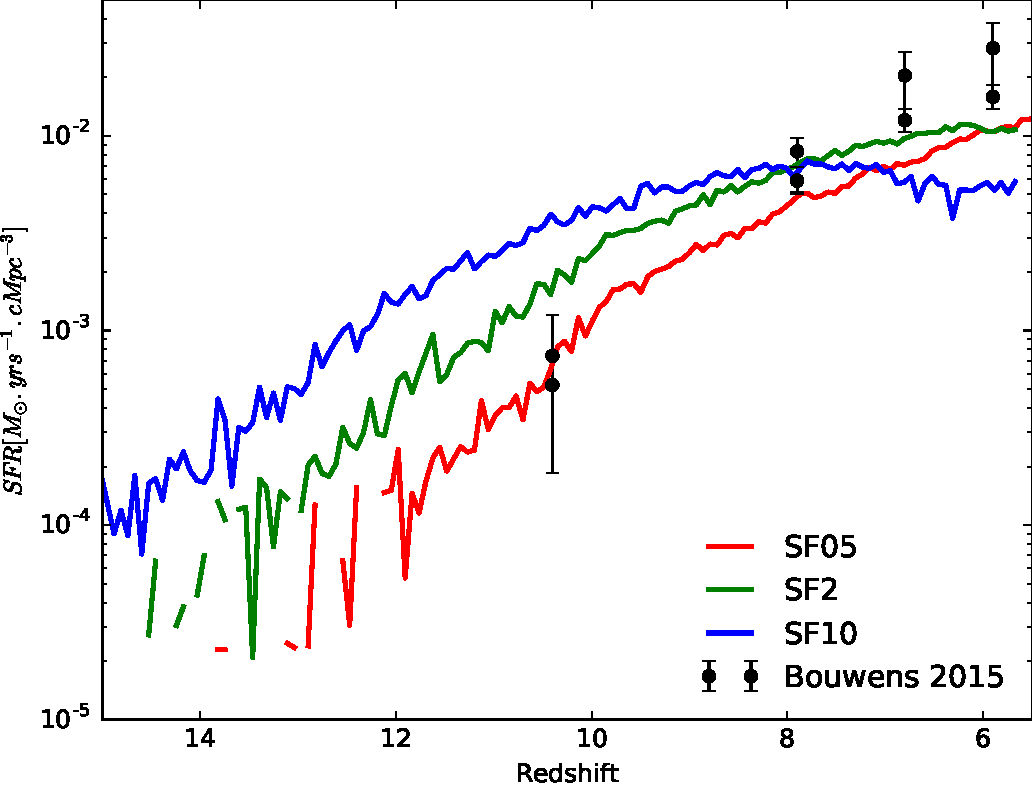
\includegraphics[width=.95\textwidth]{img/03/sedov/SFR_sfeff.pdf} 
        \caption{SFH cosmique en fonction de l'efficacité de formation stellaire.
        Toutes les simulation utilise la même méthode d'injection et la même quantité d'énergie.
		L'effet du couplage est bien présent.
        }
 		\label{fig:sfr_sfe}
\end{figure}

Une observation importante par rapport au deuxième test est qu’indépendamment de la quantité d'énergie injectée, et que même si la SFR est significativement impacté, l'histoire d'ionisation reste quasiment constante (cd fig \ref{fig:xion_sneff}).


\begin{figure}[bth]
        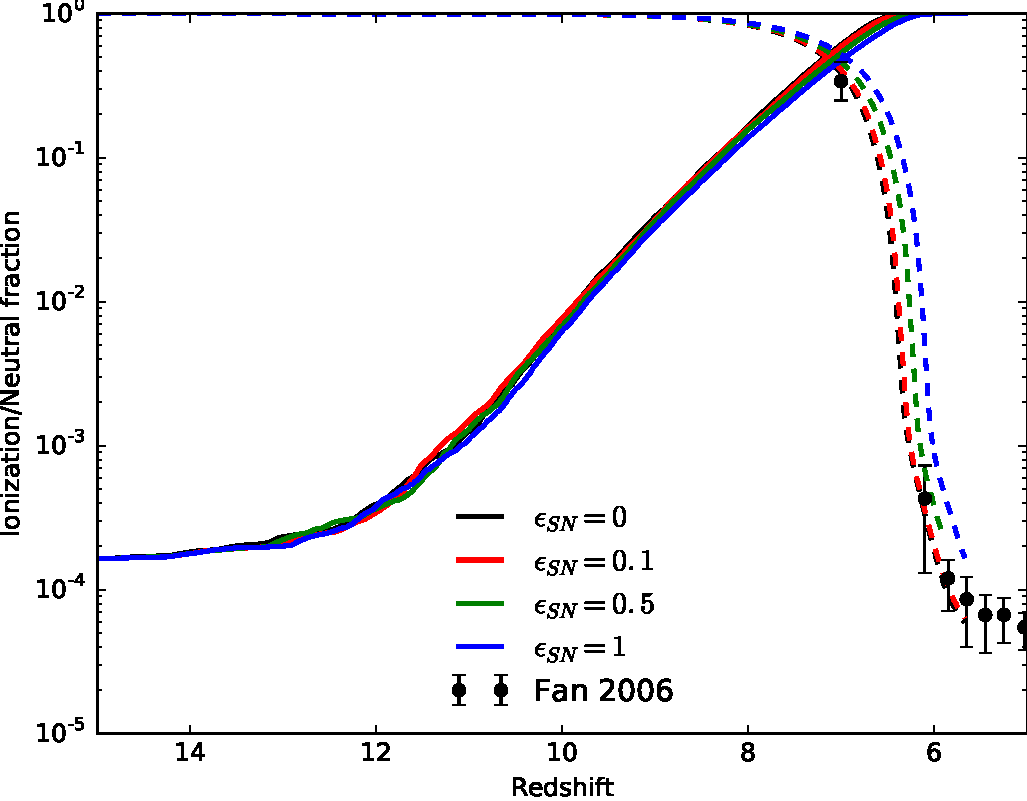
\includegraphics[width=.95\textwidth]{img/03/sneff_xion.pdf} 
        \caption{Malgré une SFH différente (voir figure \ref{fig:sfr_egy}), l'histoire d'ionisation est conservée en changeant la quantité d'énergie injectée.
        }
 		\label{fig:xion_sneff}
\end{figure}

Cet effet est inattendu car si la quantité d'étoiles diminue, la quantité de radiation diminue d'autant, et donc la fonction d'ionisation globale devrait être impacté.
Or ce n'est pas ce qui est observé ici.
Dans le but d'explorer cet effet, nous allons nous concentrer dans la suite a une étude galaxies par galaxies.











